\documentclass[12pt, a4paper]{article}

% Acentuação
\RequirePackage[T1]{fontenc}
\RequirePackage[utf8]{inputenc}

% Configurando as margens
\usepackage[top = 2cm, bottom = 2cm, left = 3cm, right = 3cm]{geometry}
% Indentação do parágrafo
\setlength{\parindent}{2cm}
% Espaçamento entre parágrafo e texto
\setlength{\parskip}{1em}
% Espaçamento entre linhas
\renewcommand{\baselinestretch}{1.5}
% Identar o primeiro parágrafo das seções
\usepackage{indentfirst}
% Para usar símbolos como >=
\usepackage{amssymb}
% Para colocar texto entre $$ com \text{oi}
\usepackage{amsmath}
% Para usar listas com estilos específicos
\usepackage{enumerate}
% Para utilizar imagens
\usepackage{graphicx}
% Posicionamento de imagem
\usepackage{float}
% Para múltiplas linhas em tabelas
\usepackage{multirow}
% Para \ang{30} - símbolo de ângulo °
\usepackage{siunitx}

\renewcommand{\figurename}{Figura}
\renewcommand{\tablename}{Tabela}

\begin{document}

	\title{Fundações I - Resumo}
\date{\today}
\author{@ivansnpmaster}
\maketitle

	\section{Fundações rasas ou diretas (superficiais)}

		\subsection{Bloco de fundação}
		Os blocos são elementos de fundação de grande rigidez, executados com concreto simples ou ciclópico (portanto, não armado), dimensionado de tal forma que as tensões de tração neles produzidas, sejam absorvidas pelo próprio concreto.

*Inserir imagens

$$A=a\cdot b$$ $$A=\frac{P}{\sigma_s}$$ $$h=\frac{a-a_0}{2}\cdot \tan{\alpha}$$

*Inserir imagens

Onde $a$ é o maior lado do bloco, $b$ é o menor lado do bloco, $a_0$ é o maior lado do pilar, $b_0$ é o menor lado do pilar, $P$ é a carga do pilar, $\sigma_s$ é a tensão admissível do solo, $h$ é a altura do bloco, $\alpha$ é o ângulo interno e $\sigma_t$ é a tensão admissível de tração do concreto.

*Inserir ábaco

O valor de $\alpha$ é obtido através do ábaco, entrando-se com o valor $\sigma_s/\sigma_t$, em que $\sigma_s$ é a tensão que o bloco aplica ao solo (carga do pilar + peso próprio do bloco, dividido pela área da base) e $\sigma_t$ é a tensão admissível de tração do concreto, que é da ordem de $f_{ck}/25$ e não é recomendável adotar valores superiores a 0,8 $MPa$.

Exemplo: Dimensionar um bloco de fundação sujeito a uma carga de 1700 $kN$, aplicada por um pilar de (35x60) $cm$, executado com concreto com $f_{ck}$ de 15 $MPa$, sobre um solo com taxa igual a 0,4 $MPa$. Desprezar o peso próprio.

O primeiro passo é determinar a área da base, portanto: $$A=\frac{P}{\sigma_s}=\frac{1700\;kN}{0,4\;MPa}=\frac{1700\;kN}{400\;\frac{kN}{m^2}}=4,25\;m^2$$

Como o pilar é retangular, é interessante ter um bloco da mesma forma. Como a $\sqrt{4,25}$ é próxima de 2, estima-se um valor abaixo disso para $b$, a fim de encontrar um valor para $a$ um pouco maior que 2. Portanto, estima-se um $b=1,9\;m$ e o outro lado ($a$) é $4,25\;m^2/1,9\;m\approx 2,25\;m$. Note que o valor dessa divisão foi arredondado para cima, e isso deve ser feito objetivando medidas de 5 em 5 $cm$ (para facilitar a confecção de fôrmas).

Então, determina-se a altura do bloco. Para isso, precisa-se verificar se a tensão admissível de tração do concreto está dentro do limite estabelecido:

$$\sigma_t=\frac{f_{ck}}{25}=\frac{15\;MPa}{25}=0,6\;MPa < 0,8\;MPa$$

O valor está dentro do limite, podemos prosseguir. Agora, deve-se encontrar o ângulo interno do bloco através do ábaco. Primeiramente, verifica-se a seguinte relação: $$\frac{\sigma_s}{\sigma_t}=\frac{0,4\;MPa}{0,6\;MPa}\approx 0,67$$

A relação fornece um $\alpha$ de $\ang{60}$ pelo ábaco. Deve-se verificar a altura em ambas as direções ($a$ e $b$) da peça, como prossegue:

$$h_a=\frac{a-a_0}{2}\cdot \tan{\alpha}=\frac{2,25-0,6}{2}\cdot \tan{\ang{60}}\approx 1,45\;m$$
$$h_b=\frac{b-b_0}{2}\cdot \tan{\alpha}=\frac{1,9-0,35}{2}\cdot \tan{\ang{60}}\approx 1,35\;m$$

Novamente os valores foram arredondados para cima, no mesmo padrão de 5 em 5 $cm$. Adota-se o maior valor de $h$ entre $h_a$ e $h_b$. O bloco de fundação tem $a=2,25\;m$, $b=1,9\;m$ e $h=1,45\;m$.



		\subsection{Sapatas}
		São elementos de fundação executados em concreto armado com altura reduzida em relação às dimensões da base e caracteriza-se, principalmente, por trabalhar à flexão.

Tipos de sapatas:

\begin{itemize}
	\item Sapata isolada;
	\item Sapata conjugada ou viga de fundação;
	\item Sapata corrida;
	\item Sapata com viga de equilíbrio ou sapata com viga alavanca;
	\item Sapata associada ou radier parcial.
\end{itemize}

\subsubsection{Sapata isolada}

São aquelas que atendem a um único pilar.

\begin{figure}[htb]
	\begin{center}
	\caption{Sapata isolada em perpspectiva.}
    	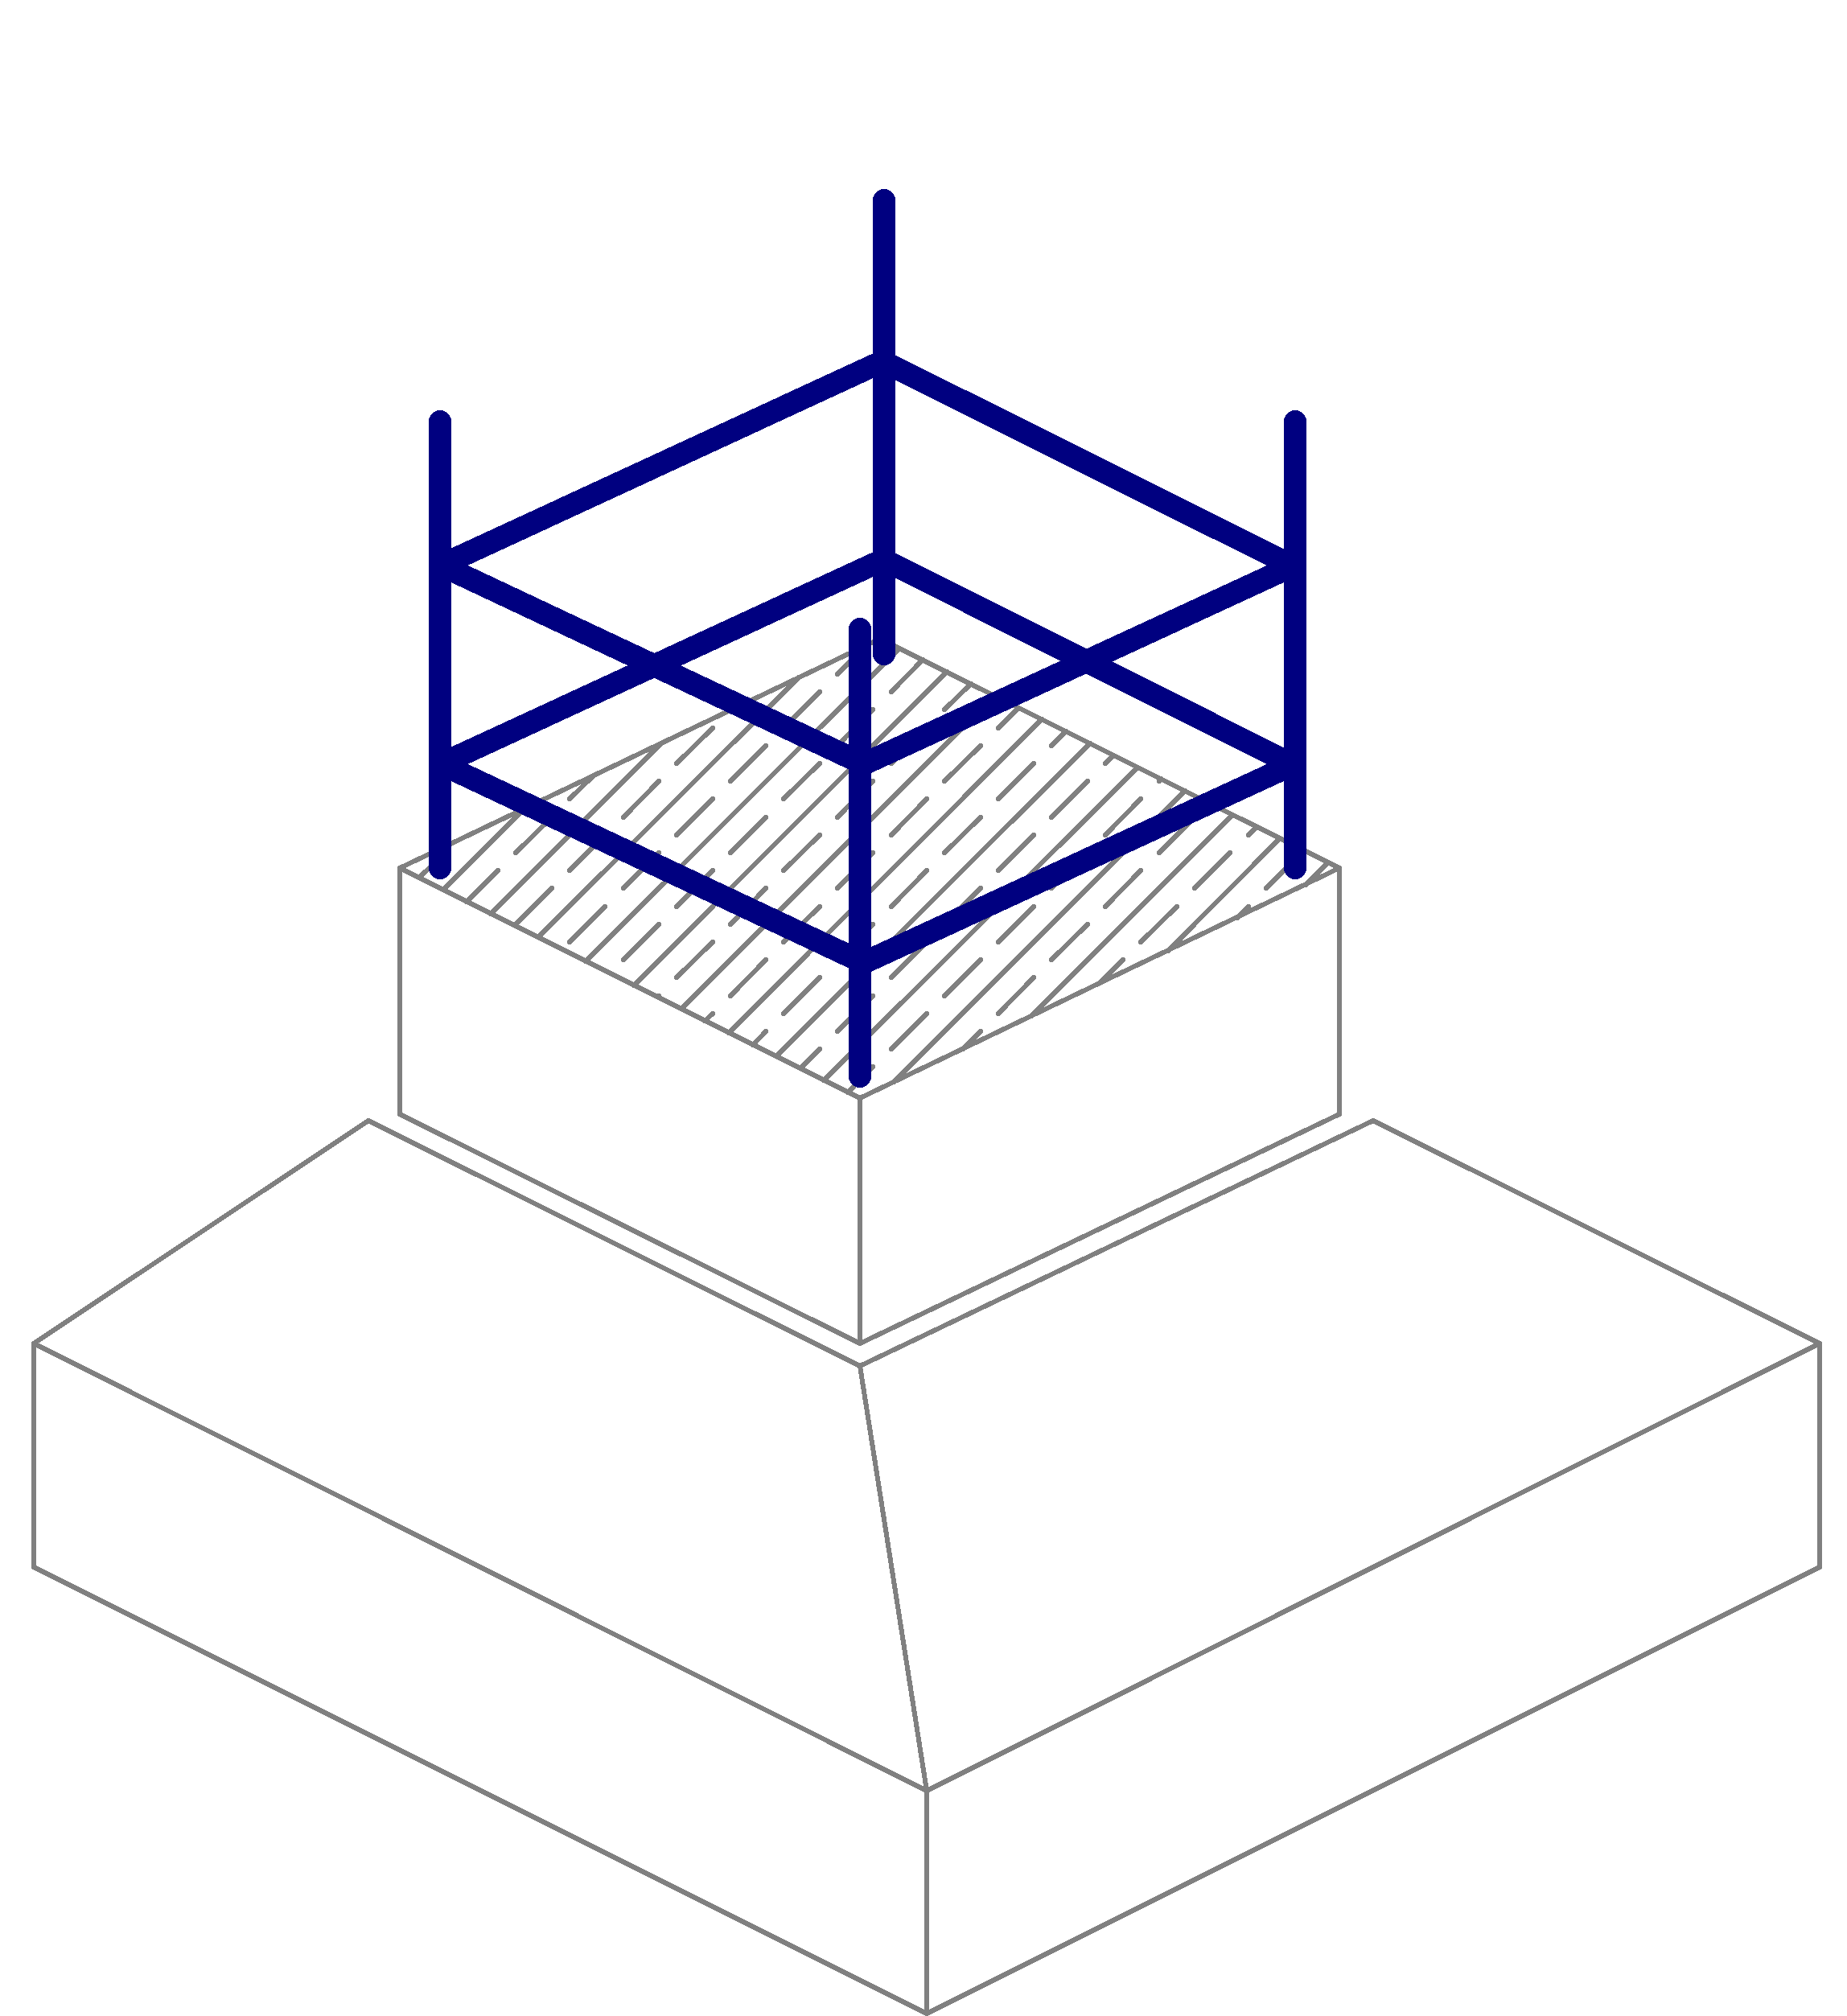
\includegraphics[width=0.4\textwidth]{Fundacoes-rasas-ou-diretas/Imagens/Sapata-isolada-1.png}
	\end{center}
\end{figure}

Para o pré-dimensionamento de altura de uma sapata, pode-se utilizar a seguinte equação:

\begin{equation}
	h=30\%\cdot a
\end{equation}

Alguns \textbf{critérios de projeto} devem ser considerados no pré-dimensionamento de sapatas isoladas:

\begin{enumerate}
	\item O centro de gravidade da sapata deverá coincidir com o centro de carga dos pilares; $${CG}_{sapata}={CG}_{pilar}$$
	\item Nenhuma dimensão da sapata deverá ser inferior a 60 $cm$; $$b\geqslant60\;cm$$
	\item A relação entre os lados da sapata não deverá ultrapassar a 2,5; $$\frac{a}{b}\leqslant2,5$$
	\item Os balanços da sapata deverão ser iguais nas duas direções ortogonais da peça. $$a-a_0=b-b_0$$
\end{enumerate}

Observações:

\begin{enumerate}
	\item Quando o somatório das áreas das sapatas ultrapassar 50\% da área da projeção da edificação no terreno, deve-se trocar a solução \textbf{sapata isolada} por \textbf{radier};
	\item Ao escolher o tipo de fundação a ser adotado em um projeto, deve-se testar, \textbf{primeiramente}, a solução \textbf{sapata isolada}. Caso não seja possível, deve-se partir para outras alternativas, inclusive \textbf{fundações profundas}.
\end{enumerate}

A figura a seguir ilustra o caso de \textbf{sapatas em terrenos inclinados}. Percebe-se que uma nova sapata deve ficar no mínimo a uma distância $b$ da sapata já construída.

*Inserir imagem

Exemplo: Dimensionar as sapatas para os pilares P1 e P2 com as seguintes características:
P1 (30x30) $cm\rightarrow$ 3000 $kN$; P2 (30x60) $cm\rightarrow$ 4200 $kN$; $\sigma_s=0,3\;MPa$.

Para \textbf{P1}:

Como $a_0=b_0$, a sapata será quadrada ($a=b$). $$A=b\cdot b$$ $$A=b^2$$

Como $A=\frac{P}{\sigma_s}$, tem-se:

$$b=\sqrt{\frac{P}{\sigma_s}}=\sqrt{\frac{3000\;kN}{300\;\frac{kN}{m^2}}}\approx3,162\;m\approx3,2\;m$$

Portanto, a altura $h$ da sapata é $h=30\%\cdot a=30\%\cdot 3,2=0,96\approx0,95$

Nota-se que foi arredondado para baixo. Pode-se fazer isso quando os arredondamentos de $a$ e $b$ forem mais folgados e consequentemente não atrapalharem na quantidade de área. Se fosse utilizado $h=0,95\;m$, fazendo a conta inversa, obteria-se um $a=0,95/0,3\approx3,17\;m\approx3,2\;m$.

Para \textbf{P2}:

O pilar é retangular, indicando que as dimensões da sapata também serão.
$$A=\frac{P}{\sigma_s}=\frac{4200\;kN}{300\;\frac{kN}{m^2}}=14\;m^2$$

Como $A=a\cdot b$:
$$a=14\;m^2/b$$

Para que os momentos fletores sejam iguais nas duas direções ortogonais, tem-se:
$$a-a_0=b-b_0$$
$$\frac{14}{b}-0,6=b-0,3$$

Multiplicando todos os elementos por $b$:
$$14-0,6b=b^2-0,3b$$

Igualando toda a equação a zero, tem-se:
$$b^2+0,3b-14=0$$

Encontrando-se as raízes por Bhaskara:
$$x_{1, 2}=\frac{-b\pm\sqrt{b^2-4\cdot a\cdot c}}{2\cdot a}=\frac{-0,3\pm\sqrt{0,3^2-4\cdot 1\cdot (-14)}}{2\cdot1}$$
$$x_1\approx3,59\;m$$
$$x_2\approx-3,89\;m$$

Voltando, tem-se:
$$a=\frac{14\;m^2}{b}=\frac{14\;m^2}{3,59\;m}\approx3,89\;m\approx3,9\;m$$

Percebe-se que as duas raízes da equação correspondem aos lados da sapata, sendo uma delas em módulo. A altura $h$ é, portanto:
$$h=30\%\cdot a=30\%\cdot 3,9\;m=1,17\;m\approx1,2\;m$$

As dimensões das sapatas isoladas são: P1 ($a=b=3,2\;m$ e $h=0,95\;m$); e P2 ($a=3,9\;m$, $b=3,6\;m$ e $h=1,2\;m$).

		\subsection{Sapatas com seção "L", "U" e "Z"}
		Para pilares com seções mais complexas, deve-se obter um pilar retangular equivalente, de modo que se possa utilizar os métodos já vistos.

\begin{figure}[H]
	\begin{center}
	\caption{Vista em planta de um pilar com seção "L".}
    	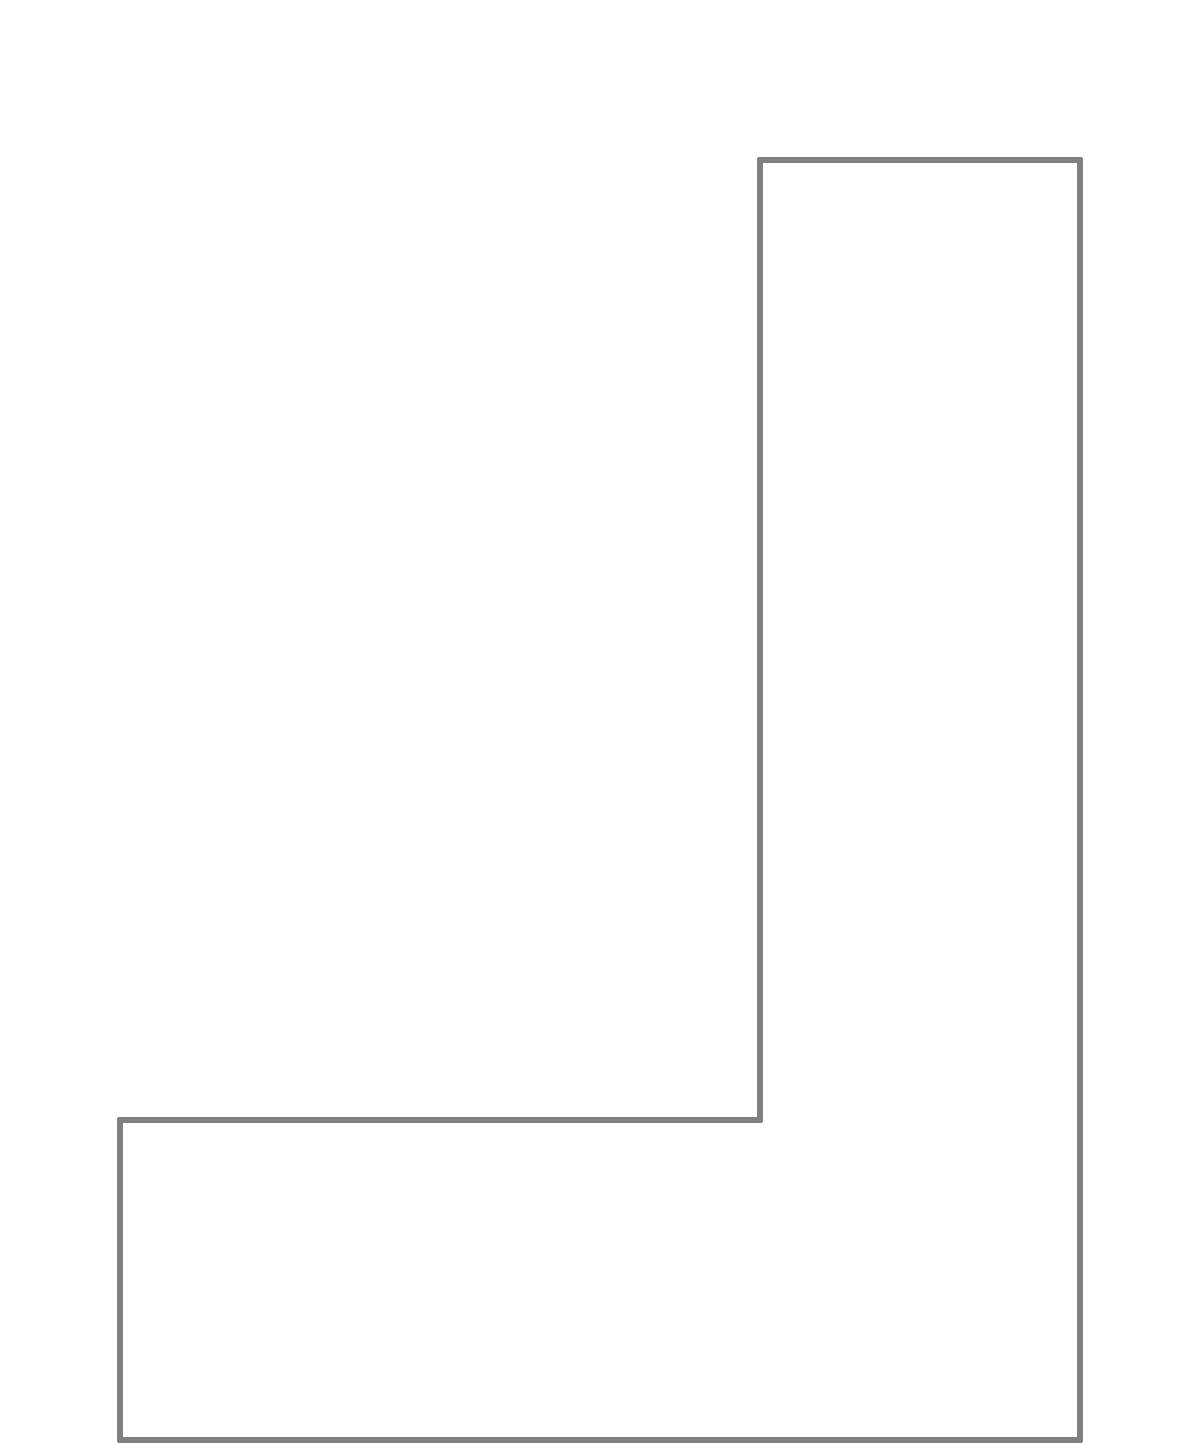
\includegraphics[width=0.25\textwidth]{Fundacoes-rasas-ou-diretas/Imagens/Sapatas-com-secao-LUZ.png}
	\end{center}
\end{figure}

O primeiro passo é subdividir a figura inicial em figuras menores de geometria conhecida (preferencialmente retangular), cada qual com seu respectivo centro geométrico (CG), como segue:

\begin{figure}[H]
	\begin{center}
	\caption{Vista em planta da subdivisão do pilar em "L" em geometrias mais simples.}
    	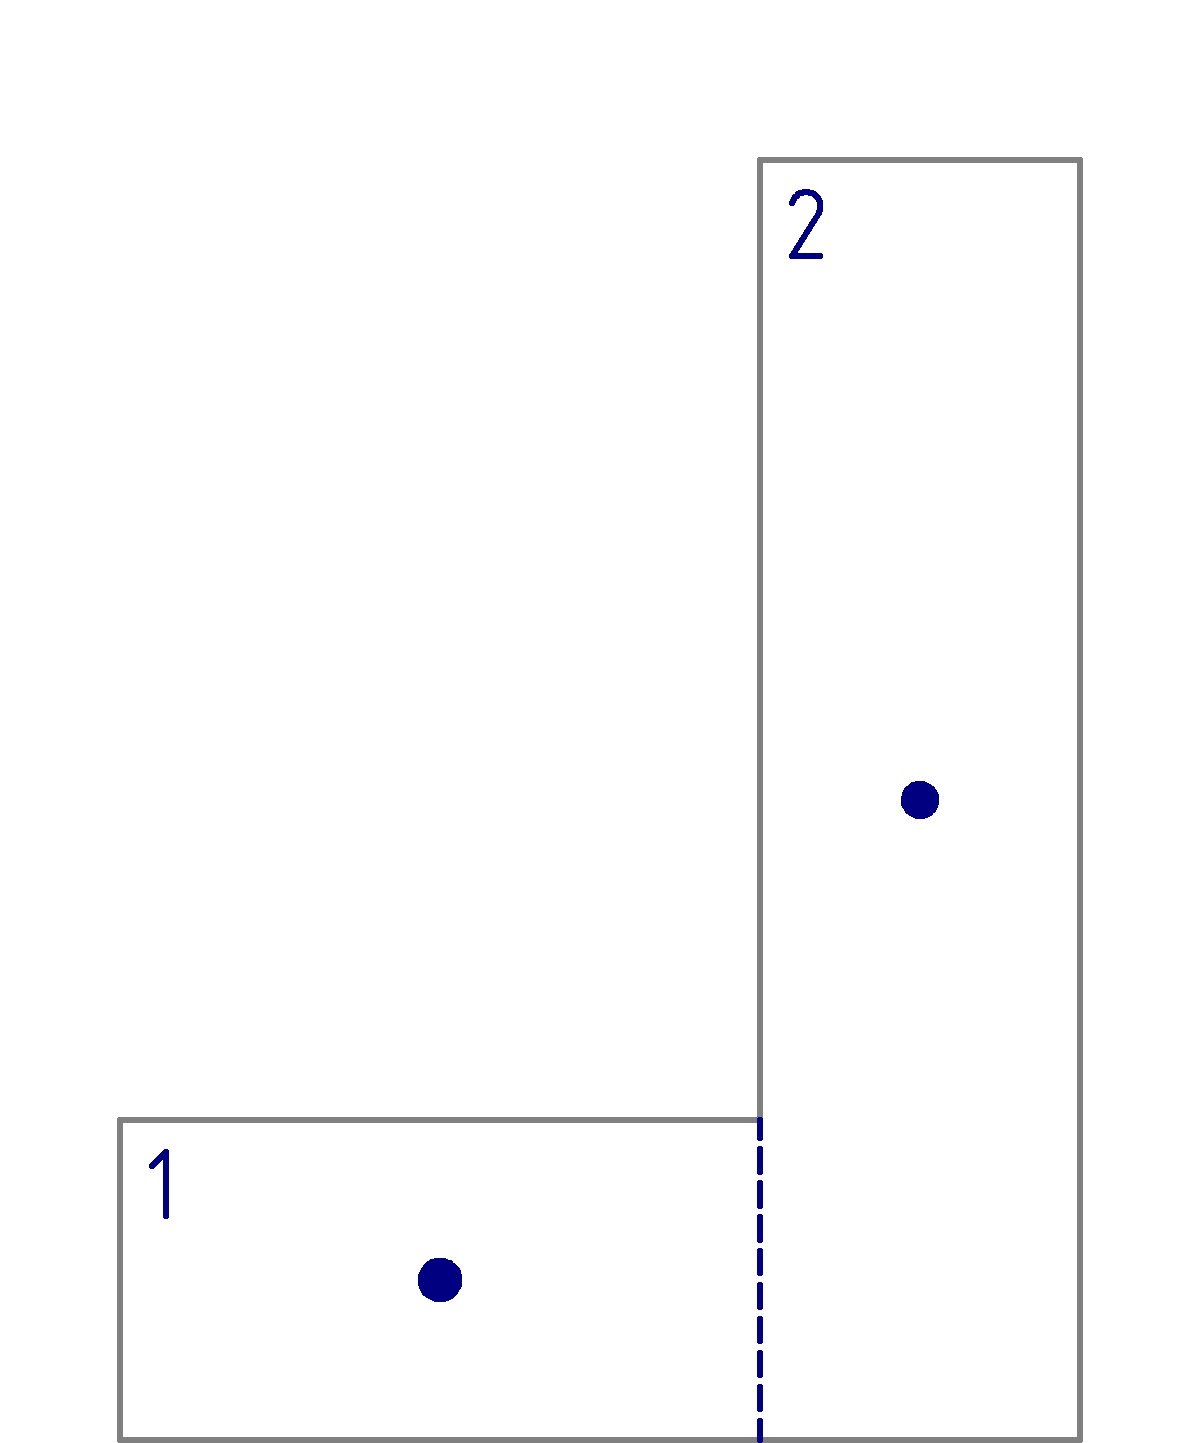
\includegraphics[width=0.25\textwidth]{Fundacoes-rasas-ou-diretas/Imagens/Sapatas-com-secao-LUZ-2.png}
	\end{center}
\end{figure}

Essa subdivisão permite o cálculo das coordenadas do CG da figura mais complexa pelas seguintes médias ponderadas:

\begin{equation}x_{CG}=\frac{\displaystyle\sum_{i=1}^{n} A_i\cdot \overline{x}_i}{\displaystyle\sum_{i=1}^{n} A_i}\end{equation}
\begin{equation}y_{CG}=\frac{\displaystyle\sum_{i=1}^{n} A_i\cdot \overline{y}_i}{\displaystyle\sum_{i=1}^{n} A_i}\end{equation}

Onde $x_{CG}$ e $y_{CG}$ são as coordenadas do CG da figura final; $A_i$ é a área da figura $i$; e $\overline{x}_i$ ou $\overline{y}_i$ é a coordenada do CG da figura fracionada $i$.

Além disso, antes de calcular os pontos de CG da figura mais complexa, coloca-se eixos de referência na figura, como segue:

\begin{figure}[H]
	\begin{center}
	\caption{Vista em planta da colocação de eixos para encontrar o CG.}
    	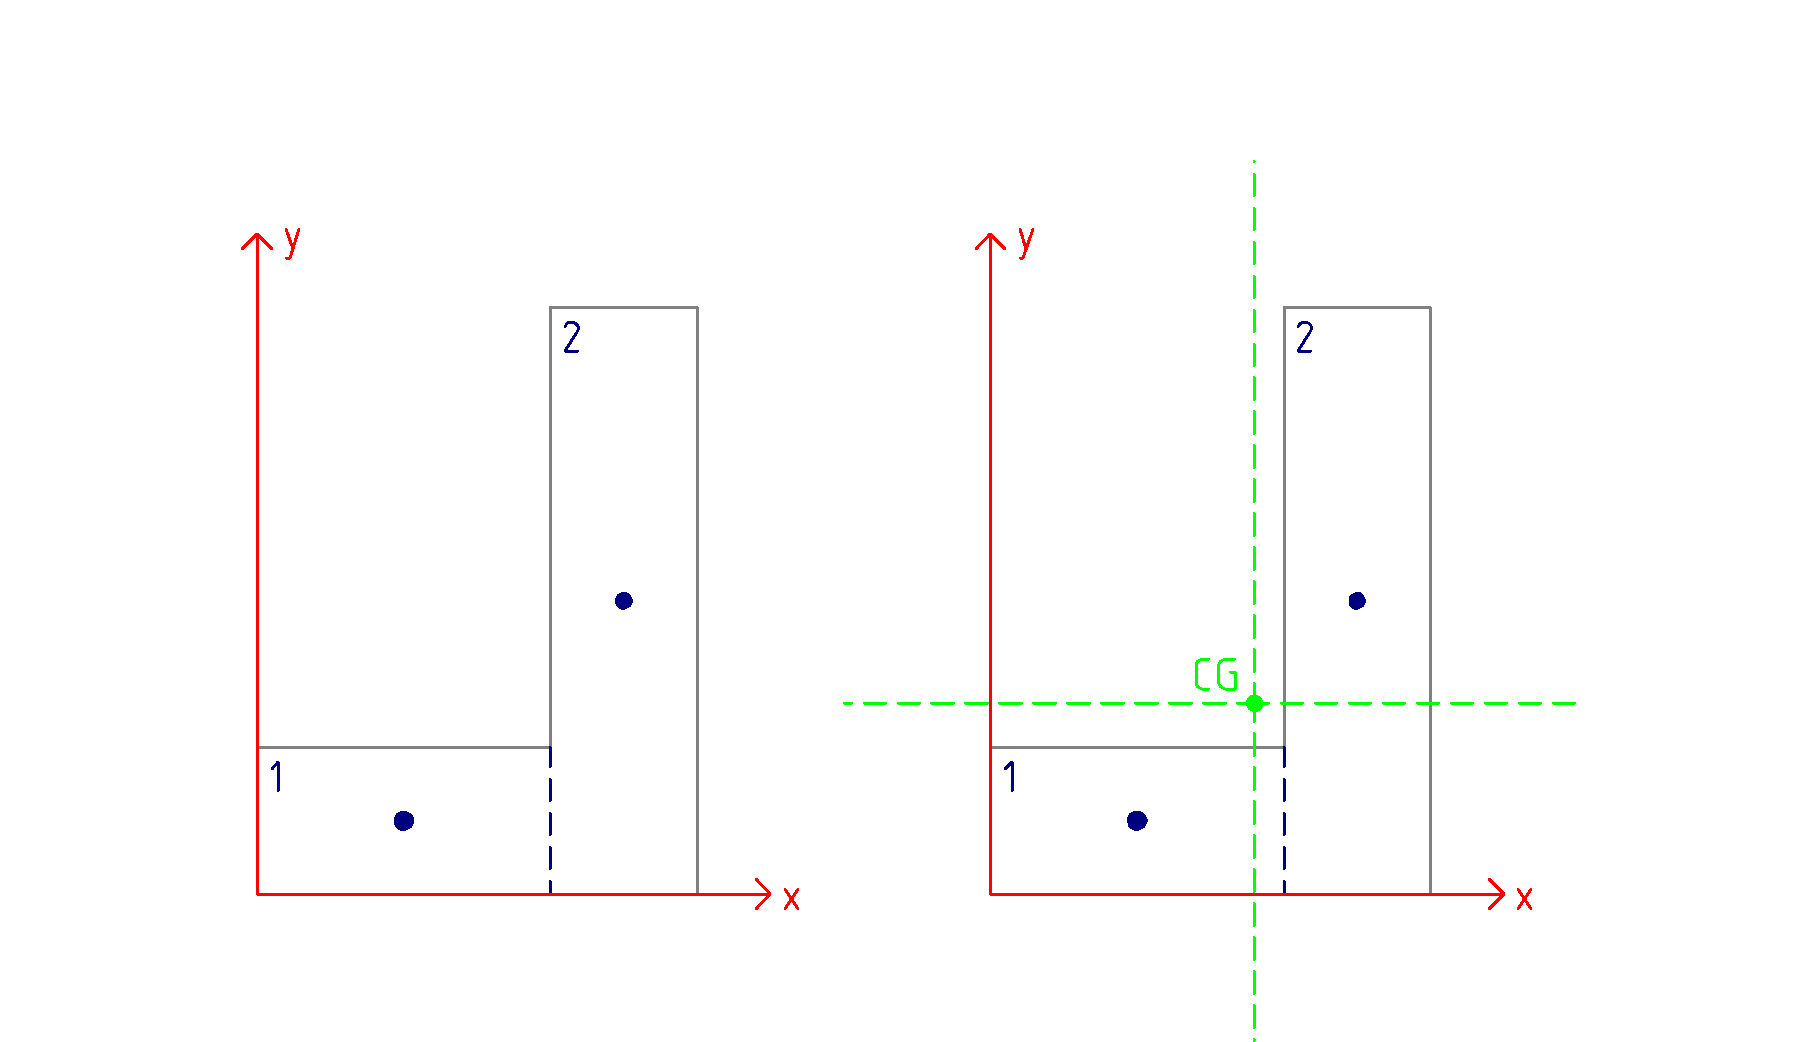
\includegraphics[width=0.85\textwidth]{Fundacoes-rasas-ou-diretas/Imagens/Sapatas-com-secao-LUZ-3.png}
	\end{center}
\end{figure}

Agora, deve-se checar, a partir dos eixos traçados, qual a maior distância de ambas as superfícies da peça em cada eixo até o ponto CG, ou seja:

\begin{figure}[H]
	\begin{center}
	\caption{Vista em planta da checagem da distância de cada extremidade em relação ao CG da figura principal.}
    	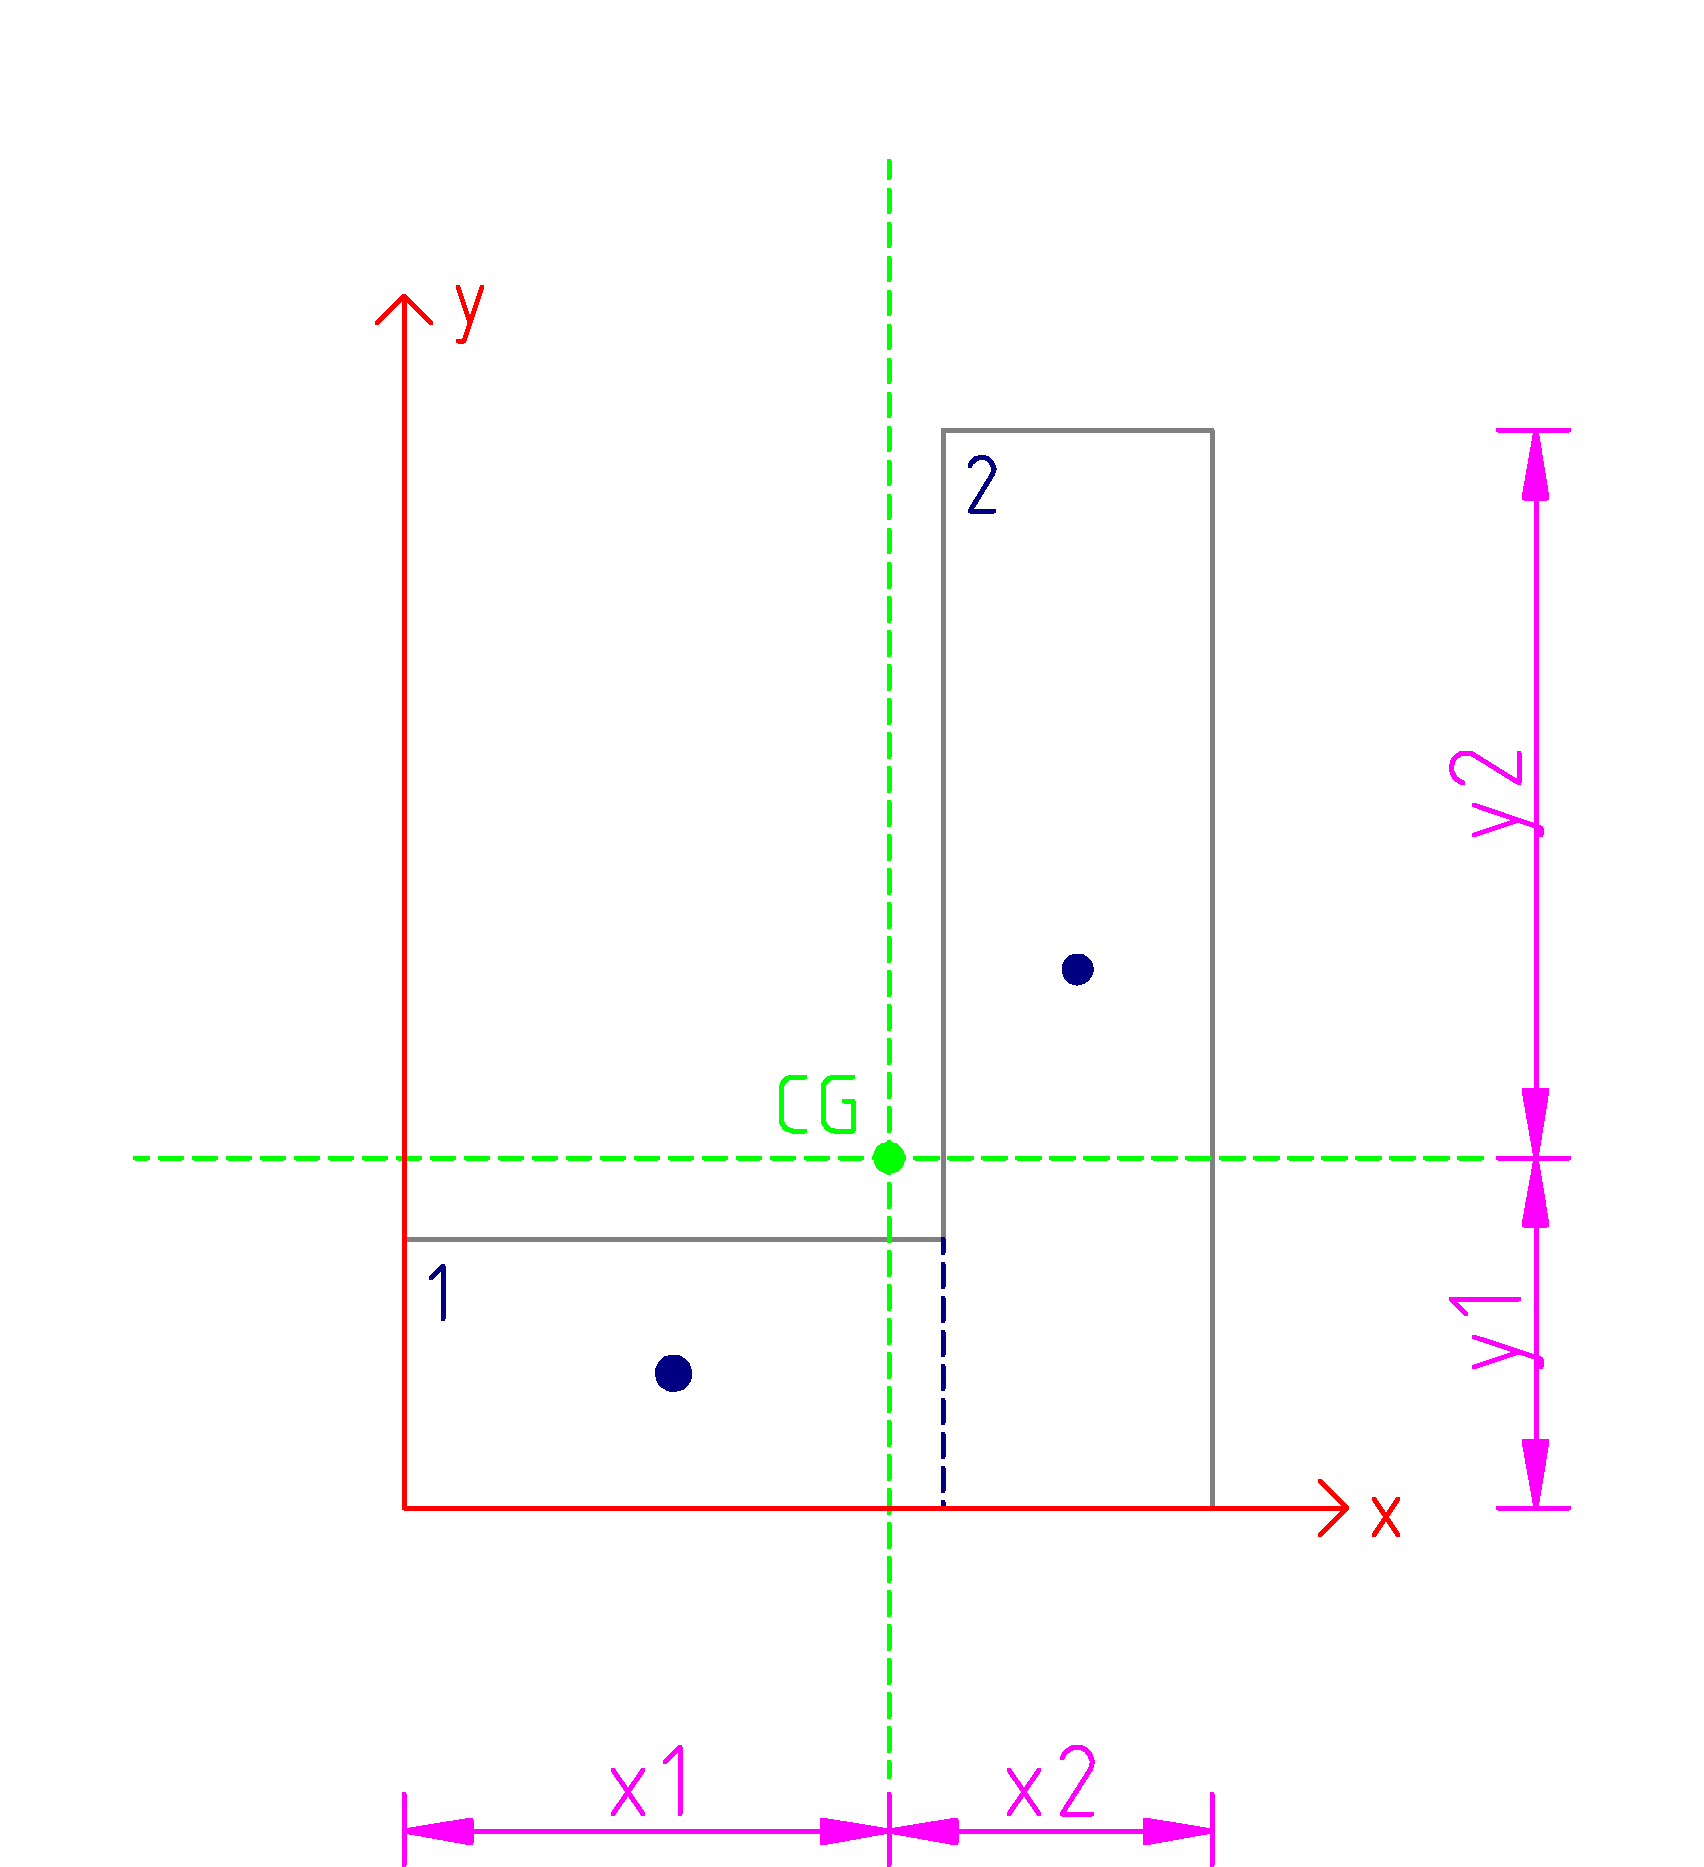
\includegraphics[width=0.45\textwidth]{Fundacoes-rasas-ou-diretas/Imagens/Sapatas-com-secao-LUZ-4.png}
	\end{center}
\end{figure}

O maior valor deve ser dobrado para cada eixo. Assim, o pilar retangular equivalente com mesmo CG é obtido.

\begin{figure}[H]
	\begin{center}
	\caption{Vista em planta dos comprimentos do pilar retangular equivalente para a seção em "L".}
    	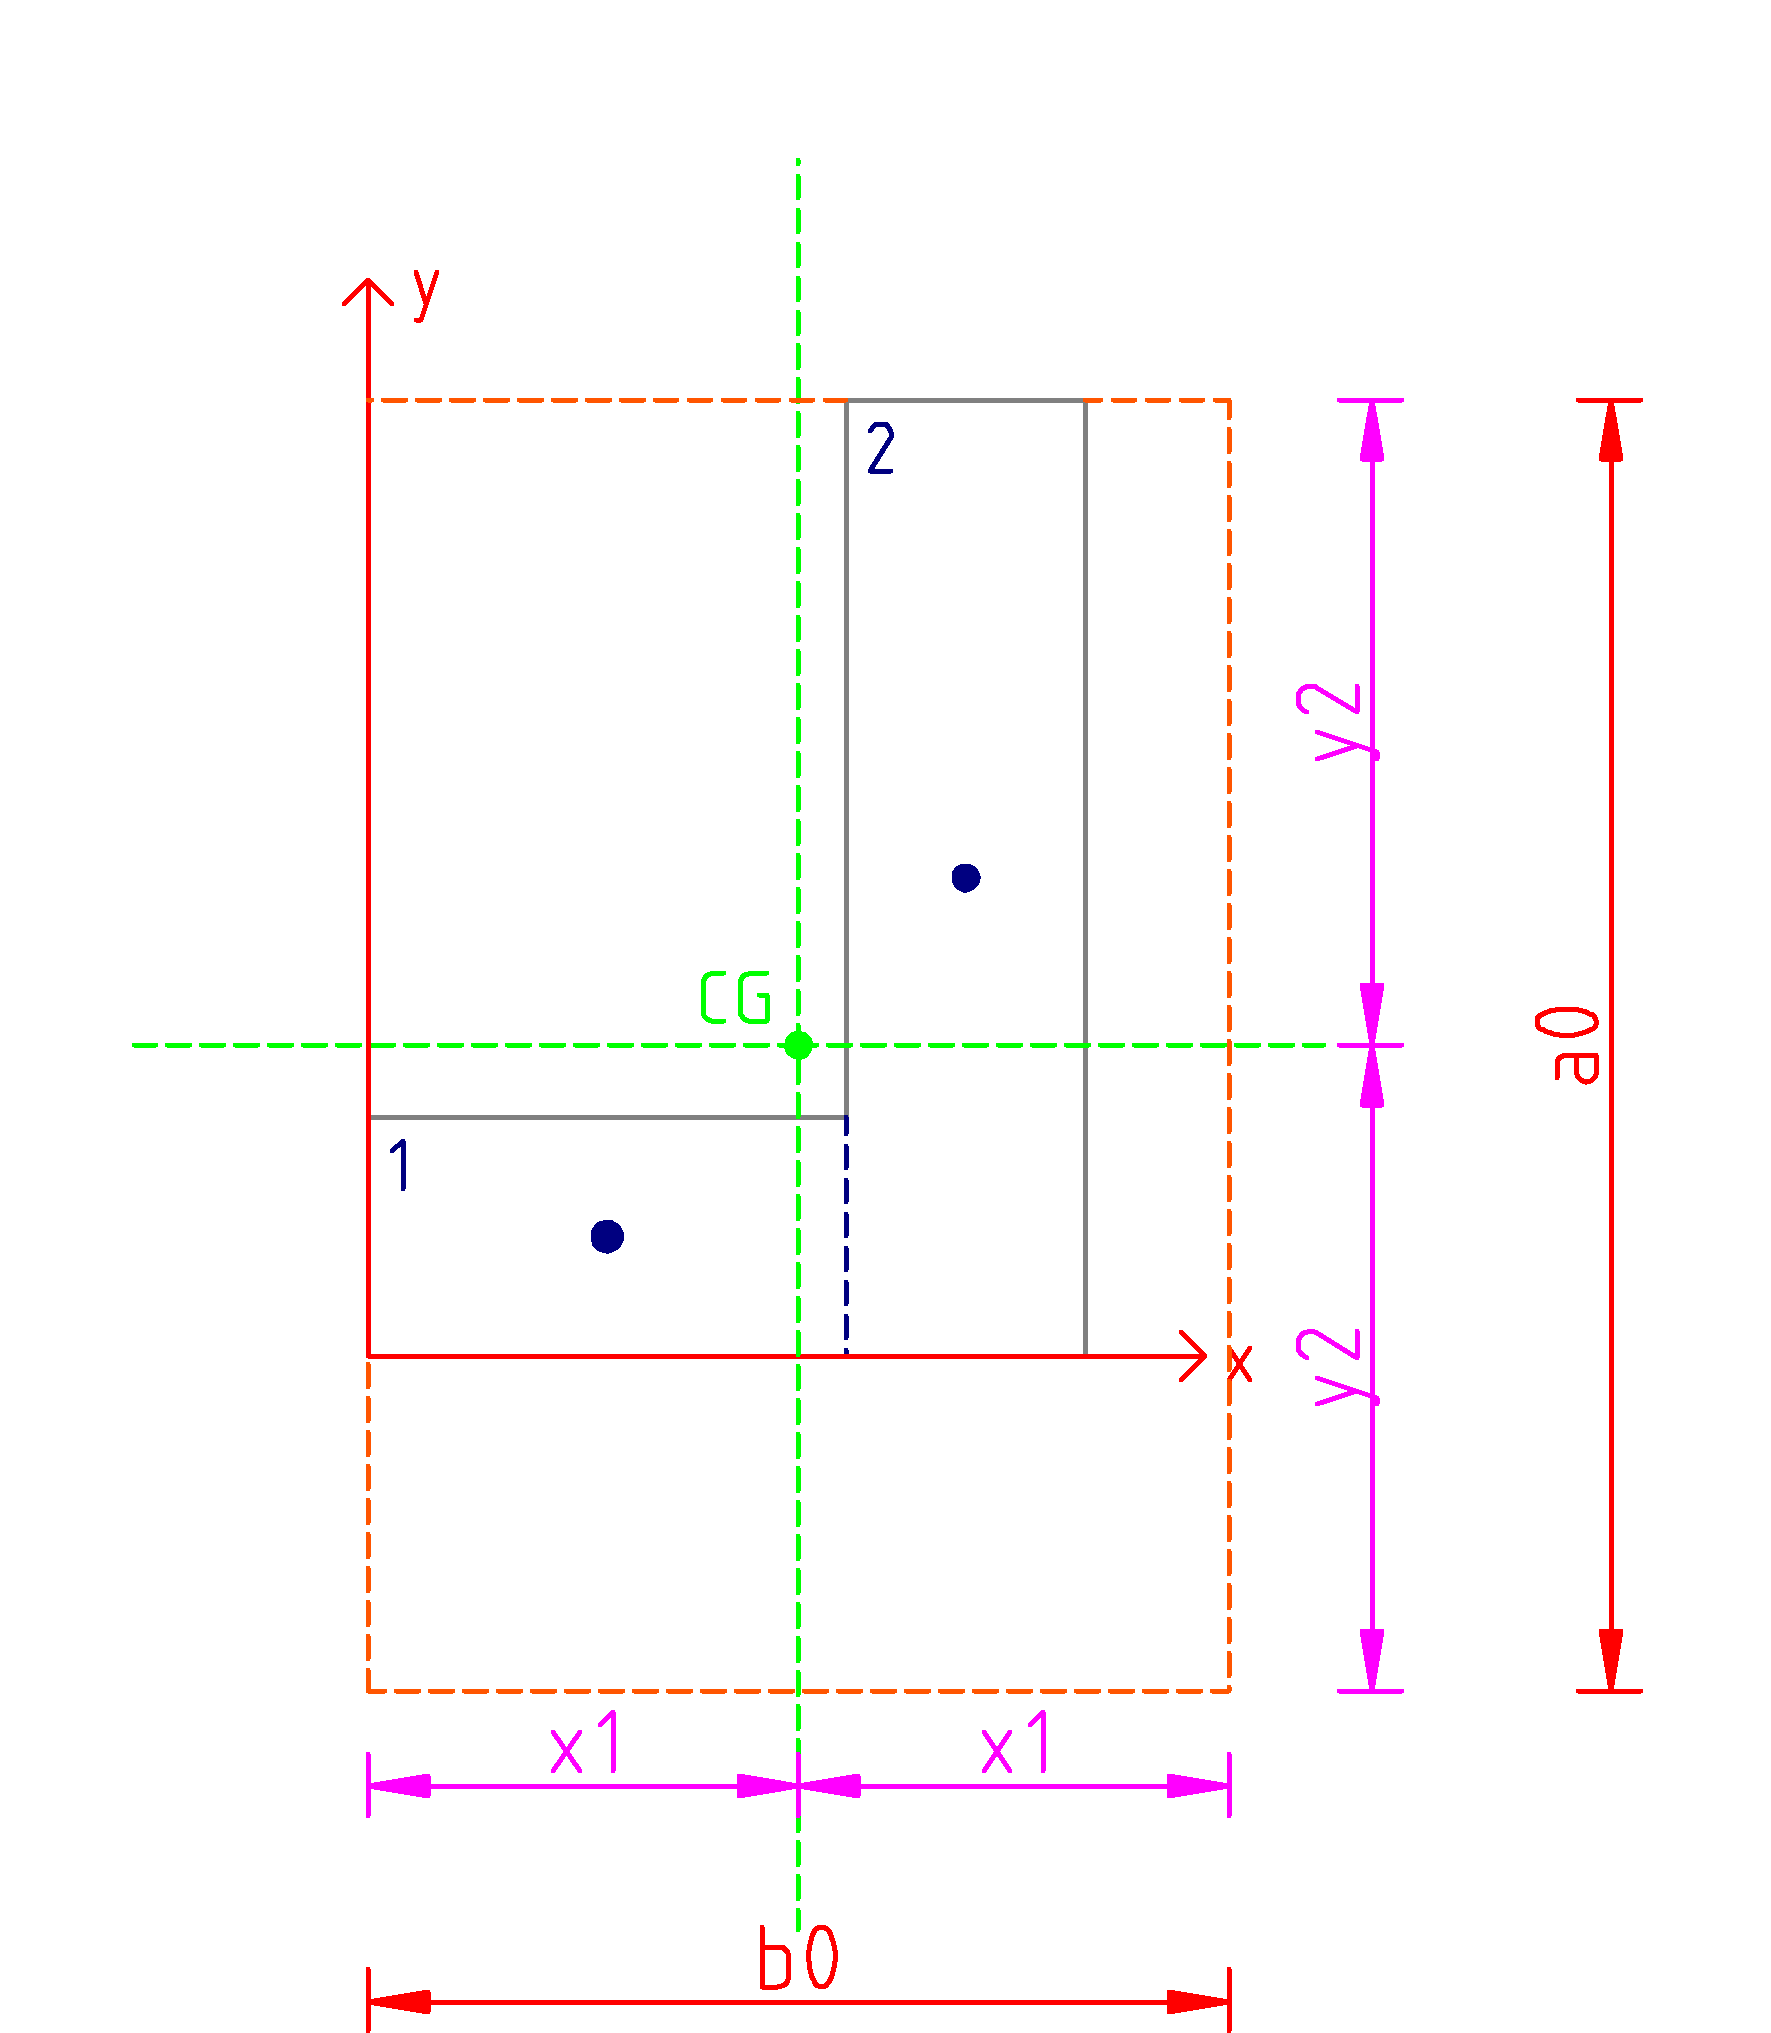
\includegraphics[width=0.45\textwidth]{Fundacoes-rasas-ou-diretas/Imagens/Sapatas-com-secao-LUZ-5.png}
	\end{center}
\end{figure}

		\subsection{Pilares com cargas distintas nos diferentes ramos}
		\begin{figure}[H]
	\begin{center}
	\caption{Pilar de elevador com cargas distintas nos diferentes ramos.}
	\label{figura-pilar-de-elevador-cargas-distintas}
    	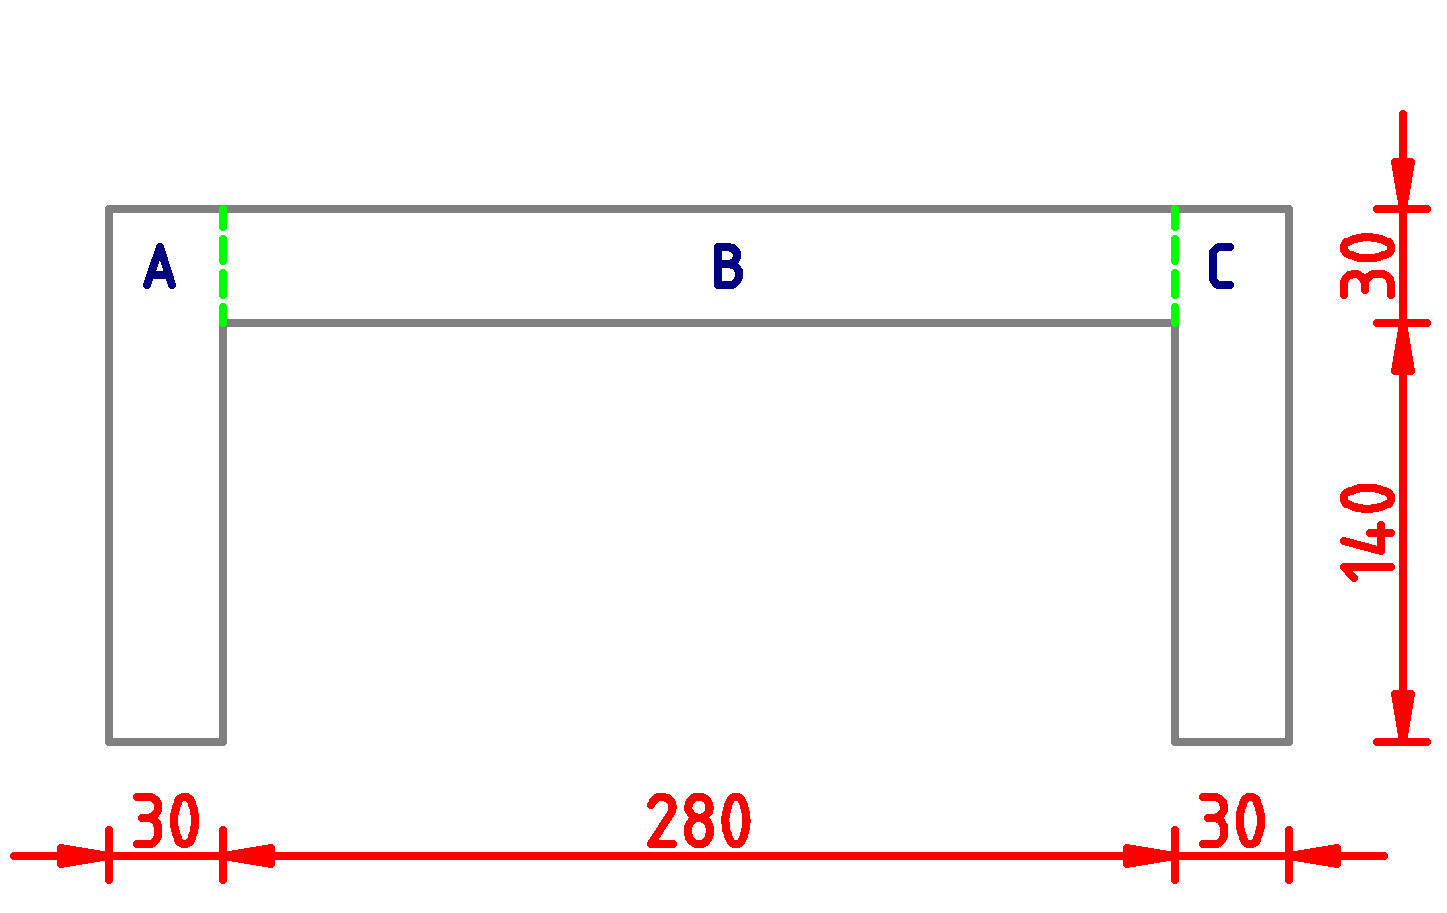
\includegraphics[width=0.4\textwidth]{Fundacoes-rasas-ou-diretas/Imagens/Pilares-com-cargas-distintas-nos-diferentes-ramos.png}
	\end{center}
\end{figure}

Cargas: $A=5000\;kN/m^2$, $B=6000\;kN/m^2$ e $C=7000\;kN/m^2$.

Deve-se montar um pilar retangular fictício onde o seu centro de carga (CC) coincida com o centro de carga do pilar da Figura~\ref{figura-pilar-de-elevador-cargas-distintas}. Encontra-se o ponto de centro de carga baseado numa média ponderada das cargas de cada ramo, como segue:
\begin{equation}
	\label{equacao-xcc}
	x_{CC}=\frac{\displaystyle\sum_{i=1}^n P_i\cdot \overline{x}_i}{\displaystyle\sum_{i=1}^n P_i}
\end{equation}
\begin{equation}
	\label{equacao-ycc}
	y_{CC}=\frac{\displaystyle\sum_{i=1}^n P_i\cdot \overline{y}_i}{\displaystyle\sum_{i=1}^n P_i}
\end{equation}

O primeiro passo é converter as cargas que estão por $m^2$ em cargas pontuais, ou seja, o produto entre a carga por $m^2$ e a área da respectiva peça:
$$\text{A}=5000\;kN/m^2\cdot(0,3\;m\cdot1,7\;m)=2550\;kN$$
$$\text{B}=6000\;kN/m^2\cdot(2,8\;m\cdot0,3\;m)=5040\;kN$$
$$\text{C}=7000\;kN/m^2\cdot(0,3\;m\cdot1,7\;m)=3570\;kN$$

A carga total $P$ é, portanto:
$$P=2550\;kN+5040\;kN+3570\;kN=11160\;kN$$

A coordenada $x_{CC}$ pela Equação~\eqref{equacao-xcc}:
$$x_{CC}=\frac{2550\;kN\cdot0,15\;m+5040\;kN\cdot1,7\;m+3570\;kN\cdot3,25\;m}{11160\;kN}\approx1,84\;m$$

A coordenada $y_{CC}$ pela Equação~\eqref{equacao-ycc}:
$$y_{CC}=\frac{2550\;kN\cdot0,85\;m+5040\;kN\cdot1,55\;m+3570\;kN\cdot0,85\;m}{11160\;kN}\approx1,17\;m$$

Como $x_{CC}=1,84\;m$, essa distância é a maior entre as faces das extremidades nesse eixo até o centro de carga, portanto, o valor de $a_0$ (maior lado do pilar fictício retangular):
$$a_0=2\cdot x_{CC}=2\cdot1,84\;m=3,68\;m$$

Da mesma maneira, como $y_{CC}=1,17\;m$ é a maior distância entre as faces das extremidades nesse eixo até o centro de carga, o valor de $b_0$ (menor lado do pilar fictício retangular):
$$b_0=2\cdot y_{CC}=2\cdot1,17\;m=2,34\;m$$

A área de sapata isolada necessária:
$$A=\frac{P}{\sigma_s}=\frac{11160\;kN}{300\;\frac{kN}{m^2}}\approx37,2\;m^2$$

A área necessária é, também, o produto dos seus lados. Logo, o lado $a$ é:
$$a=\frac{A}{b}=\frac{37,2\;m^2}{b}$$

Pode-se substituir o valor de $a$, $a_0$ e $b_0$ na Equação~\eqref{equacao-equilibrio-balancos}:
$$a-a_0=b-b_0$$
$$\frac{37,2}{b}-3,68=b-2,34$$

Multiplicando ambos os lados por $b$ e igualando a zero:
$$b^2+1,34\cdot b-37,2=0$$

Encontrando as raízes por Bhaskara:
$$x_{1,2}=\frac{-b\pm\sqrt{b^2-4\cdot a \cdot c}}{2\cdot a}=\frac{-1,34\pm\sqrt{1,34^2-4\cdot 1 \cdot (-37,2)}}{2\cdot 1}$$
$$x_1\approx5,46\;m\approx5,5\;m$$
$$x_2\approx-6,805\;m\approx-6,85\;m$$

Portanto, $a=6,85\;m$ e $b=5,5\;m$.

		\subsection{Sapata conjugada (ou viga de rigidez)}
		Sapata conjugada é uma estrutura de fundação que associa dois ou mais pilares, alinhados num mesmo bloco.

*Inserir figuras

A fim de se obter as coordenadas do centro de carga (CC) do sistema, coloca-se um ponto referencial no centro de carga de $P1$ e realiza-se o somatório de momentos na direção $x$ na Figura $x$, ou seja:
$$(P1+P2)\cdot x=P2\cdot d_1$$

Isolando-se $x$ [que nesse caso é o centro de carga (CC) do sistema], tem-se:
\begin{equation}x=\frac{P2\cdot d_1}{P1+P2}\end{equation}

Da mesma maneira para a direção $y$, tem-se:
$$(P1+P2)\cdot y=P2\cdot d_2$$

Isolando-se $y$:
\begin{equation}y=\frac{P2\cdot d_2}{P1+P2}\end{equation}

A área de sapata conjugada necessária é obtida a partir das cargas dos pilares e da tensão admissível do solo ou, ainda, pelo produto de seus lados:
\begin{equation}A=\frac{P1+P2}{\sigma_s}=a\cdot b\end{equation}

Pode-se classificar a sapata conjugada quanto ao posicionamento dos pilares:

\textbf{Próximos à divisa}:
\begin{itemize}
	\item Pilar mais leve fica mais próximo da divisa;
	\item Pilar mais pesado fica mais próximo da divisa;
\end{itemize}

\textbf{Afastados da divisa}:
\begin{itemize}
	\item Pilares com o mesmo carregamento;
	\item Pilares com carregamentos diferentes.
\end{itemize}

Para o \textbf{primeiro caso}, onde o pilar mais leve fica mais próxim da divisa, pode-se encontrar a coordenada $x_{CC}$ estabelecendo-se um ponto de referência $PR$ e fazendo a somatória dos momentos fletores em relação àquele ponto. Como segue:

*Inserir figura

$$x_{CC}=\frac{P1\cdot\displaystyle\frac{b_0}{2}+P2\cdot\left(d_1+\displaystyle\frac{b_0}{2}\right)}{P1+P2}$$

Para o \textbf{segundo caso}, onde o pilar mais pesado fica mais próximo da divisa, deve-se utilizar o Método do Trapézio para encontrar as dimensões do seguinte sistema:

*Inserir figura:

O Método do Trapézio é realizado da seguinte forma:
\begin{enumerate}
	\item Calcular o centro de carga;
	\item Adotar o valor de $y=x_{CC}$
		\begin{equation}x_{CC}=\frac{P1\cdot x_1+P2\cdot x_2}{P1+P2}=y\end{equation}
	\item Estimar o valor de $c$ em ($c<3\cdot y$)
	\item Calcular a área da base da sapata:
		$$A=\frac{P1+P2}{\sigma_s}$$
		\begin{equation}A=(a+b)\cdot \frac{c}{2}\end{equation}
	\item Calcular a parcela $(a+b)$:
		\begin{equation}(a+b)=\frac{2\cdot A}{c}\end{equation}
	\item Calcular o valor de $b$:
		$$y=\frac{c}{3}\cdot\left[\frac{(a+b)+b}{a+b}\right]$$
		\begin{equation}b=\left[\frac{3\cdot y}{c}\cdot(a+b)\right]-(a+b)\end{equation}
	
	Se $b<60\;cm$, retornar ao passo onde se estima o valor de $c$, diminuir o seu valor e recalcular $b$, passando pelos tópicos intermediários novamente.
	\item Calcular $a$:
		\begin{equation}a=\frac{2\cdot A}{c}-b\end{equation}
\end{enumerate}

\end{document}